\chapter{How \textsc{Becca}'s reinforcement learner works}
\label{actor_chapter}

\textsc{Becca}'s reinforcement learner starts with the set of feature activities passed from the feature extractor at each time step. (See Figure~\ref{becca_reinforcement_learner}.) It passes the full feature activities and reward to the model and chooses an action to pass to the world.

\begin{figure}
\centering
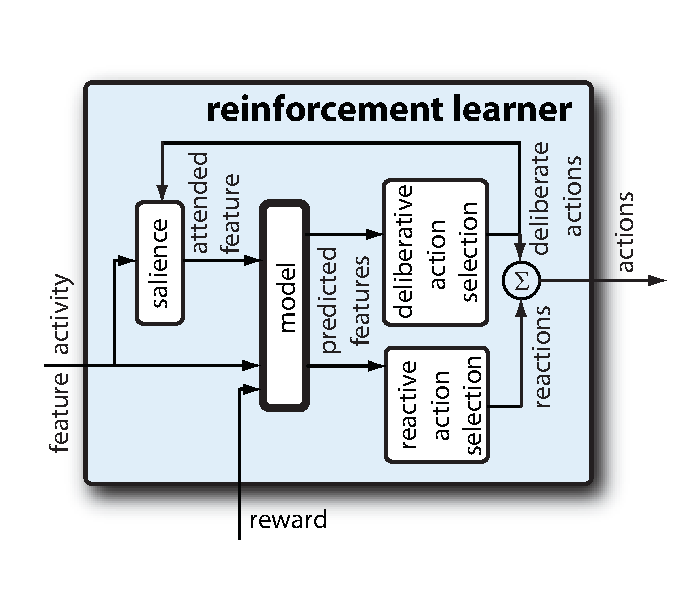
\includegraphics[height=11cm]{figs/becca_reinforcement_learner.eps}
\caption{Block diagram of \textsc{Becca}'s reinforcement learner.}
\label{becca_reinforcement_learner}
\end{figure}

\section{Model}
The model is the core of the reinforcement learner. It contains snippets of the agent's experience in the form of {\em transitions}. Taken together, the collection of transitions is a distillation of the agent's interactions with its world. On the agent's first time step, the model is empty, but as it gathers experience it gradually populates its model, increasing the fidelity of its representation of the world. 

\subsection{Transition structure}

Each transition is of the form (\texttt{context}, \texttt{cause}, \texttt{effect}, \texttt{reward}) and captures a short sequence of events. Contexts, causes, and effects may contain state or action information or both. Transitions also contain a quantification of the uncertainty in both effects and rewards. \texttt{context}--\texttt{cause} pairs uniquely define a transition. The effect and reward that results from a given context feature and cause feature may vary a great deal each time the transition is observed. Rewards and effects are the expected value of starting in a given context and executing a given cause. The reward uncertainty and effect uncertainty are the expected error on those predictions.

\subsubsection{Context}
Context, $\mathbf{c}$, is a recently active feature. Specifically, if the current time step is labeled $t$, any one of the set of active features at $t-1$ may be the context of a relevant transition. 

\subsubsection{Cause}
Cause, $\mathbf{d}$, is a currently active feature. It may be an action, in which case the \texttt{context}--\texttt{cause}--\texttt{effect} sequence resembles a state--action--state tuple. But it can also be a primitive feature or created feature, in which case the transition represents an observed sequence of features, rather than a record of the agent's interaction with the world

\subsubsection{Effect}
The effect, $\mathbf{e}$, is the set of expected feature activities for a given \texttt{context}--\texttt{cause} pair. It is updated using the full set of feature activities from time $t$. It contains the cause, but also all the other features that tend to result from that context and cause.

\subsubsection{Effect uncertainty}
Each time a transition is observed, the effect is updated to reflect the result. It can be the case that a wide variety of effects may result from the same context and cause. The effect captures something resembling the average of these effects. The effect uncertainty provides an estimate of the expected difference between the effect and effects that will result from future encounters with the same context and cause. Taken together, the effect value and uncertainty provide a coarse characterization of the probability distribution of effects. The effect uncertainty is useful in assessing the agent's confidence in its predictions.

\subsubsection{Reward}
The reward that results from each observation of the transition is used to update an estimate of the transition's expected reward. This quantity explicitly describes the desirability of the transition.

\subsubsection{Reward uncertainty}
As with the effect, the reward uncertainty is the expected value of the difference between the expected reward and future observations of reward. Taken together, the reward value and uncertainty provide a coarse characterization of the probability distribution of rewards. It is also a quantification of confidence in the reward estimate.

\subsubsection{Count}
The count is a reflection of the number of times a transition has been observed. It determines the update rate for transitions.

\subsection{Transition updates}
The effect, reward, and their uncertainties for each transition are updated based on their similarities to the new observation. 

When a transition is updated, the following events occur:
\begin{itemize}
\item The reward is normalized.
\item The count is increased.
\item The effect is modified to incorporate the newly observed effect.
\item The effect uncertainty is modified to incorporate the difference between the effect and the newly observed effect.
\item The reward is modified to incorporate the newly observed reward.
\item The reward uncertainty is modified to incorporate the difference between the reward and the newly observed reward.
\end{itemize}

The range of the reward is tracked the same way as the sensor values in the previous Appendix, and the value is normalized to fall in the desired range:

\begin{eqnarray}
\hat{r}_{\max}^{\prime} &=& \max \left ( \hat{r}_{\max}, \hat{r} \right ) \\
\hat{r}_{\min}^{\prime} &=& \min \left ( \hat{r}_{\min}, \hat{r} \right ) \\
r &=& \frac{\hat{r} -  \hat{r}_{\min}}{\hat{r}_{\max} -  \hat{r}_{\min}}
\end{eqnarray}

The extremes of each range are gradually contracted as well, to account for drift.

\begin{eqnarray}
\hat{r}_{\max} &=& \hat{r}_{\max} - D_{rrr} ( \hat{r}_{\max} -  \hat{r}_{\min}) \\
\hat{r}_{\min} &=& \hat{r}_{\min}  + D_{rrr} (\hat{r}_{\max} -  \hat{r}_{\min}) 
\end{eqnarray}


For the transition associated with context $c_i$ (any context with feature $i$ active) and cause $d_j$ (any cause with feature $j$ active):

\begin{equation}
\sigma = (f_{i_{t - 1}} f_{j_t}) ^ {D_{mex}}
\end{equation}

where $D_{mex}$ is typically a small integer and $f_{i_t}$ is the activity of feature $i$ at time $t_0$. $\sigma$ is close to one if the context feature was active on the prior time step and the cause feature is active on the current time step. 

In order to perform the updates, an update rate, $\rho_e$ is first calculated:

\begin{equation}
\rho_e = \min \left (\frac{1}{2}, \sigma \left ( D_{tur}+ \frac{1 - D_{tur}}{n} \right ) \right )
\end{equation}
        
where $n$ is the count of the transition being updated and $D_{tur}$ is a real value between zero and one. For large values of $n$, $\rho_e$ approaches $D_{tur}$. It can be considered a lower bound on the update rate. For values of $D_{tur}$ close to zero, transitions cease to change significantly after they have been observed many times. For higher values of $D_{tur}$, they remain malleable throughout their lifetimes.

Each feature in the effect is updated, shifted toward the newly observed value by a fraction of the way, $\rho_e$. For an existing effect feature value, $e_i$, and a new effect observation $\tilde{e}_i$ the updated feature value, $e^\prime_i$ is given by:

\begin{eqnarray}
\Delta e_i &= &\tilde{e}_i  - e_i \\
e^\prime_i &=& e_i + \rho_e \Delta e_i
\end{eqnarray}

By the same mechanism, the effect uncertainty features, $e_{\epsilon_i}$, are updated using $\Delta e_i$:

\begin{eqnarray}
\Delta e_{\epsilon_i} &=& |\Delta e_i|  - e_{\epsilon_i}\\
e_{\epsilon_i}^\prime &=& e_{\epsilon_i} + \rho_e \Delta e_{\epsilon_i}
\end{eqnarray}

Reward, $r$, and reward uncertainty, $r_\epsilon$ are updated using the same mechanism as well, with the same update rate:

\begin{eqnarray}
\Delta r &= &\tilde{r} - r \\
r^\prime &=& r + \rho_e \Delta r \\
\Delta r_\epsilon &=&|\Delta r| -  r_\epsilon \\
r_\epsilon^\prime &=& r_\epsilon + \rho_e \Delta r_\epsilon
\end{eqnarray}

Initially, the values for $\mathbf{e}_{\epsilon}$ and $r_{\epsilon}$ are all set to $D_{iun}$. 

Finally, the count of each transition is updated by its similarity to the current observations.

\begin{equation}
n^{\prime} = n + \sigma
\end{equation}


\subsection{Forgetting}
Every potential transition is represented in the model, but many transitions are observed only rarely. To decay and eventually forget rarely occurring transitions, the count is decremented:

\begin{equation}
n^\prime = n - \min \left ( \frac{1}{n D_{atc}}, n \right )
\end{equation}

where $n^\prime$ is the decayed count and $D_{atc}$ is a user selected constant, typically large. The nonlinear nature of the decay is such that count values above 5 or 10 will decay very slowly, but low count values will decay more quickly. This is designed to retain repeatedly-observed transitions, even if they haven't been seen in some time. This formulation for memory degradation is intended to degrade rarely-observed transitions more rapidly than those that have been observed several times.  

\section{Action selection}

The action selection method in this version of \textsc{Becca} is entirely new. At each time step, a feature is chosen to be a goal. If that feature happens to be an action, then that action is executed. There are three factors that contribute to the selection of a feature to be a goal:

\begin{enumerate}
\item Reward votes: The feature is expected to result in reward.
\item Goal votes: The feature is expected to result in a goal feature.
\item Exploration votes: The feature has not often been selected as a goal in that situation.
\end{enumerate}

These factors are combined, together with some random variation, and the feature with the highest vote is selected as the goal for that time step.

\subsection{Reward votes}

The reward portion of the feature vote comes from performing a weighted average over all matching transitions of the expected reward. For action selection, the similarity between the current feature activity and the context of each transition is of interest. For transitions with a strong match and a high expected reward, their causes show which goals are likely to result in reward. 

To calculate this, first the similarity between the current feature activity and each transition is found:

\begin{equation}
\sigma = \left ( \sum_i c_i f_i \right ) ^{D_{mex}}
\end{equation}

Then, a sample reward from each transition is calculated by randomly selecting a value from the estimated reward distribution:

\begin{equation}
\check{r} = \mathcal{U}[r - r_{\epsilon},r + r_{\epsilon})
\end{equation}

where $ \mathcal{U}$ is the uniform probability distribution over the specified interval.
In order to ensure that the action selection process is well behaved, $\check{r}$ is forced to fall between 0 and 1.

\begin{eqnarray}
\check{r} &=& \min(\check{r}, 1) \\
\check{r} &=& \max(\check{r}, 0)
\end{eqnarray}
    
Then a weighted average over all transitions calculates the expected reward associated with each of the cause features, $\phi_r$.

\begin{equation}
\phi_r = \frac{\sum \check{r} \frac{\sigma d} {r_{\epsilon}}}{\sum \frac{\sigma d} {r_{\epsilon}}} 
\end{equation}

Weighting the average by $\sigma$ emphasizes only the transitions that match the current circumstances. Weighting by $d$ masks all but the cause feature in each transition. And weighting by $1 / r_{\epsilon}$ heavily emphasizes transitions for which the reward uncertainty is low.

\subsection{Goal votes}

The goal-based portion of the vote is calculated just like the reward vote, but with a couple of modifications. Before doing this, however, the goal set updated to reflect achieved goal features and is decayed slightly.

\begin{equation}
\mathbf{g} = \mathbf{g}(1 - \mathbf{f})(1 - D_{gdr})
\end{equation}

where $\mathbf{g}$ is the set of goal values associated with the features and $D_{gdr}$ is the goal decay rate. When a feature is active, it is considered to have achieved any goal associated with it.
 
The first step in estimating the goal value associated with each transition is to find sample effect values:

\begin{eqnarray}
\check{e} &=& \mathcal{U}[e - e_{\epsilon},e + e_{\epsilon}) \\
\check{e} &=& \min(\check{e}, 1) \\
\check{e} &=& \max(\check{e}, 0)
\end{eqnarray}

These are then scaled by individual goal values and combined within a transition to get the sample goal value for that transition:

\begin{equation}
\check{g} = h( \sum_i h^{-1}(g_i \check{e}_{j_i}))
\end{equation}

where  $h(\cdot)$ is a function that maps the interval $[0, \infty)$ onto $[0,1)$:

\begin{equation}
h(x) = 1 - \frac{1}{x + 1} 
\label{inf_to_one_map}
\end{equation}

It's inverse function, $h^{-1}(\cdot)$ performs the reverse mapping:

\begin{equation}
h^{-1}(x) = \frac{1}{x} - 1
\label{one_to_inf_map}
\end{equation}

The uncertainties on the goal values of each transition are calculated similarly.

\begin{equation}
g_{\epsilon} = h \left ( \sum_i h^{-1}(g_i e_{\epsilon_i}) \right )
\end{equation}

The goal vote, $\phi_r$, is calculated using the same form of weighted average as with the reward.

\begin{equation}
\phi_g = \frac{\sum \check{g} \frac{\sigma d} {g_{\epsilon}}}{\sum \frac{\sigma d} {g_{\epsilon}}} 
\end{equation}

\subsection{Exploration votes}

The agent performs a certain amount of exploration in its interaction with its environment. Also termed ``intrinsic motivation'', ``active learning'', ``goal exploration'', and ``directed exploration'',  exploration can be driven by the how well the agent can predict the results of its actions and the behavior of its environment. 

The exploration vote associates a value with the amount of information expected to be gained by selecting a feature as a goal. In this case, it is assumed that the most information can be gained from features that have been least often observed as causes.

The weighted average of the count gives the count associated with each feature:

\begin{equation}
n_i =   \frac{\sum n \sigma d}{\sum \sigma d} 
\end{equation}

The exploration vote associated with each feature, $\phi_x$, is given by:

\begin{equation}
\phi_x = \min \left ( \frac{1 - \tilde{r}}{i_{\max} (n_i + 1) \mathcal{U}[0, 1)} , 1 \right )
\end{equation}

where $\tilde{r}$ is the current reward and $i_{\max}$ is the number of features. This formulation tends to choose goals that have not often been observed to follow the current set of features. The random quantity in the denominator permits the vote to occasionally become large, regardless of the other factors present. Larger numbers of features ($i_max$) and larger current reward tent to suppress it.

\subsection{Voting}

The reward votes, goal votes, and exploration votes for each feature are combined and used to select a goal. The index of the new goal feature is given by: 

\begin{equation}
i_{g^{\prime}} = \arg \max_i (\phi_r + \phi_g + \phi_x) (1 - \mathbf{g})
\end{equation}

The $ (1 - \mathbf{g})$ term decreases the tendency to select a goal that is already active. The magnitude of the new goal falls on $[0, 1]$ and is given by 

\begin{equation}
g^{\prime}_{i_{g^{\prime}}} = h( h^{-1}(\phi_r) + h^{-1}(\phi_g) + h^{-1}(\phi_x))
\end{equation}

After the goal is chosen, any nonzero action feature goals are identified and become the action command for that time step. Action commands are always rounded up to have a magnitude of 1.


\section{Constant values}

The values of the constants used in this version of \textsc{Becca} are listed in Table~\ref{actor_constants}. As with the feature extractor, its performance is quite sensitive to some of them.

\begin{table}[htdp]
\caption{Values used for reinforcement learner constants.}
\begin{center}
\begin{tabular}{|l|c|l|}
\hline
constant & value & description\\
\hline
$D_{rrr}$ & $10^{-10}$ & reward range decay rate\\
$D_{mex}$ & 4 & matching exponent\\
$D_{tur}$ & 0.1& transition update rate\\
$D_{iun}$ & 0.5 & initial uncertainty \\
$D_{atc}$ & $10^6$ & aging time constant \\
$D_{gdr}$ & 0.1 & goal decay rate \\
\hline
\end{tabular}
\end{center}
\label{actor_constants}
\end{table}%


